So far we have introduced a type system and process calculus for writing and checking runtime that conforms to the import mechanism for polynomial runtime.
In this section, we show that NomosUC can realize any arbitrary ITM configuration, as possible in UC, and that we can easily encode the set of fundamental proofs and lemmas of the framework and a generic composition operator.
The main challenges we overcome in realizing arbitrary ITM systems is grappling with the parent-child relationship between processes (and the provider-client reationship in channels) that prevents cyclical topologies in the normal case. 
We introduce a simple construction called \emph{providerless channels} which relies on shared session types and uses our virtual token construction. 
Second we discuss how the dummy lemma, a composition operator, and the composition theorem can be realized by the introduction of \emph{providerless channels}.

\subsection{Capturing the UC Computation Model}
The ITM computational model is extremeley flexible to capture as universal a setting as possible.
Channels in NomosUC are linear, created by some process known as the provider, and impose a strict parent-child relationship between processes. 
For example, in Figure~\ref{fig:pandq}, $P$ and $Q$ can not be connected like this with linear channels. 
Some other process $S$ must spawn either $P$, become a client of its channel, and then $P$ spawns $Q$ and becomes a client of its channel. $Q$ can never get $P$'s channel that $S$ holds due to linearity.
We overcome this constraint by introducing \emph{providerless channels} using \emph{communicator processes} that rely on shared session types~\cite{balzer2017manifest}.
We will unpack these terms one by one.

Communicators offer channels with a shared session type and acts as a buffer betweek two processes.
Shared channels can have many clients so $P$ and $Q$ can both send messages to each other through the buffer.
The communicator has the following polymorphic type:

\vspace{-1mm}
{\centering
\parbox{0cm}{
\begin{tabbing}
$\m{comm[\tau]\{n\}} = \up \echoice{$\=$ \textcolor{red}{\getpot^n} \mb{push}: \m{\tau} \arrow \m \down \m{comm[\tau]},$\\
\>$\textcolor{red}{\getpot^0} \mb{poll}: \ichoice{$\=$\textcolor{red}{\paypot^{n-1}} \mb{yes}: \m{\tau} \;\product \down \m{comm[\tau]},$\\
\>\>$\textcolor{red}{\paypot^0} \mb{no}: \; \down \m{comm[\tau]}}}$
\end{tabbing}}
\par}

\todo{where do we introduce the write-tokem, we must do it}
The new constructors $\up$ and $\down$ indicate an acquire-release paradigm so prevent non-determinism, along with the write token, when both $P$ or $Q$ attempt to write.
A senderu $P$ acquires the communicatr's channel, $\#c$, and $\mb{push}$es a functionally 
typed message along with some import $\textcolor{red}{\getpot^n}$.
The receiver $Q$ waits for $\#c$ to be released and asks for a new message with $\mb{poll}$. 
If a new message was written, $Q$ receives label $\mb{yes}$ on $\#c$, the message, and the import.
Otherwise the channel takes the $\mb{no}$ branch.
We provide the full typing rule of shared session types in Appendix~\ref{app:typing_rules}.
\begin{figure}
	\begin{subfigure}{0.5\textwidth}
	\begin{center}
	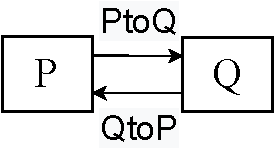
\includegraphics[scale=0.5]{figures/p_and_q.pdf}
	\caption{ITMs can communicate like this. NomosUC processes can't offer their channels to each other.}
	\label{fig:pandq}
	\end{center}
	\vspace{0.1em}
	\end{subfigure}
	\begin{subfigure}{0.5\textwidth}
	\begin{center}
	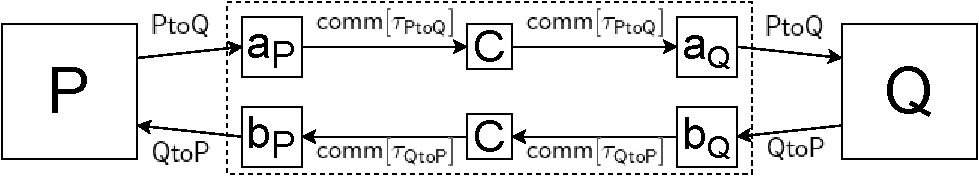
\includegraphics[scale=0.4]{figures/newPandQ.pdf}
	\caption{Processes that make up providerless channels.}
	\label{fig:newpandq}
	\end{center}
	\end{subfigure}
	\caption{Channels are labeled with their types.}
	\vspace{-1em}
\end{figure}
Communicators, alone, would constraint all processes in NomosUC to communicate through the same type $\m{comm[m]\{n\}}$, negating the descriptive session types we intended from sessio types.

We abstract normal channels into \emph{providerless channels}: a channel implemented by a communicator and some dummy processes generated at compile-time.
In Figure~\ref{fig:newpandq}, we should an illustration of a providerless channel. The dummy processes $a_P$ and $b_P$ offer the linear session types that $P$ expects and communicates with $Q$ through the communicator.
Process $a_P$ case matches on the labels in type \m{PtoQ} and sends the analogous, functionally-typed $\tau_{\m{PtoQ}}$ message to the communicator, and vice-versa for the receiving from \m{C}.
For example for \Fdb and a party (in relation to Figure~\ref{fig:newpandq}), $\m{QtoP} := \m{db}[k][v]$ and $\tau_\m{QtoP} :=$ Store \inline{of PID k v |} OK \inline{of PID |} Get \inline{of PID k |} Yes \inline{of v |} No.
Every process connected via providerless channels is wrapped in code that accepts \m{C}'s channel and spawns $a_P$ and $b_P$---thus obtaining their linear channels.
The process instantiating Figure~\ref{fig:newpandq} first spawns $C$ then $P$ and $Q$. 
The dummy processes are a trivial case statement given \m{PtoQ} and $\tau_\m{PtoQ}$ \emph{therefore, NomosUC can trivially generate them at compile-time.}
We emphasize this point as it is crucial in understanding the simpicity of composition: the key words in code are replaced by generated processes at compile-time.
\emph{In general, for the rest of this work, when we refer to processes we refer to their wrapped versions as defined by providerless channels.}

\todo{mention somewhere here that the type only accepts a constant import, but we don't care about precise time-bounds only as far as the import in the type tells the programmer what kind of computation the functionality/protocol expects to do.}
In Appendix~\ref{app:itm} we use prodiverless channels to show that NomosUC processes can realize any ITM system and vice versa (NomoUC $C' \Leftrightarrow$ ITMs $M'$).

\paragraph{\textbf{Dynamic Parties and Functionalities}}
Prior works that create security proofs or attempt some form of UC runtime analysis only do so for a statically defined number of instances of a protocol or functionality.
With providerless channels and sandboxing, NomosUC is able to overcome these limitations.
For protocol parties, we define a \partywrapper, \MX, which internally creates and runs all protocol parties, and it acts as a single endpoint for communiation with \Z, \F, and \A through two unidirectional channels each.
The channel from \MX to \F is typed with
\todo{type should have import params $n$ and $m$}
\begin{tabbing}
	$\mi{type} \; \m{P2F[\tau]\{n\}} = \ichoice{\textcolor{red}{\paypot{n}} \; \mb{p2f}: \m{PID} \arrow \m{\tau} \arrow \m{P2F[\tau]\{n\}}}$
\end{tabbing}
The protocol/functionality messages above are functionally typed, as in providerless channels, but even so, protocols and functionalities are written using their specific session type. 
On a message from \Z, \MX does
\begin{lstlisting}[basicstyle=\footnotesize\BeraMonottFamily, numbers=left, mathescape, frame=single, xleftmargin=2em, xrightmargin=2em]
$\nmatch$ $\$$z2p, $\$$f2p, $\$$a2p (
  Z2P(pid,m),*,* =>
    $\nget$ {z2pn} K $\$$z2p ;
    $\nif$ not exists pid $\nthen$
      #z2p' $\leftarrow$ channel_init[K1][z2p]; 
      $\tg{... rest of the channels ...}$
      $\$$c' $\leftarrow$ PS.prot $\leftarrow$ k rng sid 
               #z2p' #p2z' #f2p' #p2f';
      lz2p $\leftarrow$ append lz2p (pid, #z2p'); $\tg{(* store the channels *)}$
      $\tg{...}$
    $\nelse$ ()
    #z2p' $\leftarrow$ search lz2p pid ;
    $\nwithdraw$ K K1 z2pn
    #z2p'.SEND ; $\nsend$ #z2p m; $\npay$ {z2pn} K1 #z2p' ;
  *,F2P(pid,m),* => $\tg{(* identical case *)}$
  *,*,A2P(pid,m) => $\tg{(* identical case *)}$
)
\end{lstlisting}
Parties are created when their \m{PID} receives the first messages (lines 4-10). 
We reference the protocol as a module in line 7, and, as mentioned above, the providerless channels indicated by \inline{channel_init} are generated and replaced by their consituent processes before being compiled.
Finally, \MX forwards the message to the sandboxed party by creating virtual tokens and sending on its channel. 
The session type that the party receives the message through ensures that protocol ordering and import and preserved. 

Like EasyUC (and EasyCrypt), the \partywrapper acts almost like an addressing interface where messages include the receipient's \inline{PID}.
We reuse the labelling from Figure~\ref{fig:newpandq}.

An example of how the \partywrapper handles incoming messages and party creation is given in Appendix~\ref{app:arbparties}. 
As expected, sandboxing and providerless channels make the construction straightforward.

The \partywrapper construction is nearly identical to how we realize $!\F$, the multisession extension of functionalities. 
As described in Section~\ref{sec:background}, $!\F$ internally runs arbitrarily many instances of \F and multiplexes message to/from them via a subsession ID (ssid) of type \m{SID[a]} where \m{a} is functionality-specific.
For example, a common use for $!\F$ is allowing an arbitrary number of pair-wise asynchronous channels between protocol parties.
Due to the close resemblance, we do not present the code for $!\F$ here.
\todo{say something about the $!\pi$ construction?}

%%%%%%%%%%%%%%%%%%
\rmd{no more channels vs tapes}
%\paragraph*{\textbf{On Channels vs Tapes}}
%\todo{This is the passage from the paper: this modeling does not allow representing realistic
%situations where the number and makeup of components changes as the system evolves. It also does
%not capture commonplace situations where the sender has only partial information on the identity
%or code of the recipient. It also doesn’t account for the cost of message addressing and delivery; in
%a dynamically growing systems this complexity may be an important factor. Finally, it does not
%account for dynamic generation of new programs.}
%The UC framework specifically addresses prior models of distributed computation that model communication through names channels, as we do in NomosUC.
%The work suggests that though such a model is clean an elegant it doesn't allow scenarios where a sender may not have complete information about the identity or code of the receiver.
%Furthermore, it doesn't account for situations where the components in a system of ITMs evolves and changes, for example dynamic generation of new programs.
%%%%%%%%%%%%%%%%%%

\subsection{The UC Experiment}
The definition \m{execUC} is straightforward owing to our mechanism of providerless channels. 
It is a process, like any other, and offers a linear channel of type
\begin{center}
\vspace{-2mm}
\parbox{0cm}{
\begin{tabbing} 
 $\m{execout}[\K][a]\{n\} = \echoice{ \textcolor{red}{\getpot^{\{n : \K\}}}\mb{exec}: \m{Int} $\=$ \ \ichoice{ \mb{out}: \m{Bit} \product 1}}$ 
 \end{tabbing}}
\vspace{-2mm}
\end{center}
It takes, as a parameter, the security parameter $k$, a random bit string $r$ that is used as a source of randomness for all processes. 
First all channels are created, with \inline{channel_init} as above, and the first process spawned is \Z.
All \Z in NomosUC have the same type in the channel they offer to \m{execUC}:
\begin{center}
\vspace{-2mm}
\parbox{0cm}{
\begin{tabbing}
 $\m{EtoZ}[a]$ = $\m{SID}[a] \arrow [\m{PID}] \arrow \echoice{\textcolor{red}{\getpot^n} \mb{start}: \m{Bit} \arrow 1}$
 \end{tabbing}}
\vspace{-2mm}
\end{center}
It selects the session id (along with any protocol-specific parameters, \inline{a}) and the list of corrupt parties ([\m{PID}]).
\m{execUC} uses these are paramters when initializing \MX, \A, and \F.
Finally \m{execUC} $\mb{start}$s the environment with all the initial import, waits for its bit output indicating its guess for which world it is in, and forwards that bit on its own channel indicated by the type \m{execout}[a]{\n} above.
As long as the $n$ given to \m{execUC} (and so \Z) is $poly(k)$, the type system ensures the entire execution terminates in $poly(k)$.
\todo{mention how the polynomial is specified? perhaps as a parameter to \m{execUC}?}

\m{execUC} is aways parameterized by at least one virtual token type to allow for sandboxing (specifically for the \partywrapper)
and message type parameters for the protocol in question. 
It also takes in a security parameter $k$ and a random bit string $r$ that is used as a source of
randomness for all future processes.
\m{execUC} offers the following type:
The type is straightforward: the UC experiment is started with some initial amount of tokens $n$ (a user-defined parameter) and an \m{Int} security parameter, and it eventually returns the output \m{Bit} from \Z as its guess or which world it is in.
As long as $n$ is polynomial in the security parameter, the type system guarantees the execution is $poly(k)$.

%As described in the providerless channels paragraph, \m{execUC} calls a \inline{channel_init} and connects them to wrapped processes such as \inline{wrap_adv}.
%The providerless channel construction replaces these calls, with the generated portions of providerless channels.

%\m{execUC} only spawns processes already wrapped according to the providerless channel specification in Section~\ref{sec:basic}.
%Therefore, it only has to spawn the part of the channel that connects wrapped processes.
%We make this separation because the wrapped processes code is autogenerated given a specification of the session type and functional
%type associated with the process.

%All main processes in NomosUC are wrapped according to the providerless channel specification in Section~\ref{sec:basic}. 
%Therefore, \m{execUC} creates only the part of the providerless channel (e.g. $\m{PtoQ}$ channel from Figure~\ref{fig:newpandq})
%and passes them as input to the communicator wrappers.
%The wrapper creates the intermediate processes and the shared session types providing the linear channel to \m{execUC}.
%For example \Z and \A are connected by the following channels:
%\begin{lstlisting}[basicstyle=\footnotesize\BeraMonottFamily, mathescape]
%$\$$ztoa $\leftarrow$ channel_init[$\tp{G}$][$\tp{z2a}$]{$\tp{z2an}$}
%$\$$atoz $\leftarrow$ channel_init[$\tp{G}$][$\tp{a2z}$]{$\tp{a2zn}$}
%$\tg{...}$
%$\$$z <- env[G] k rng $\$$ztop $\$$ptoz $\$$ztoa $\$$atoz ;
%\end{lstlisting}

\paragraph*{\textbf{Emulation}}
The central security definition in UC is indistinguishability between the real and ideal world experiments.
It is defined in terms of the ensemble of distributions created by the output bits from the partial term
$(\m{execUC}\ \pi\ \F)$ over all possible random inputs and security parameters. 
We say that two worlds are indistinguishable if $\forall \A\ \exists \Sim\ \forall Z$
the \emph{statistical difference} in ensembles from the two worlds is negligible in $k$ (see
Definition~\ref{def:emulation} below).

\begin{definition}[Emulation]\label{def:emulation}
If two protocols $(\pi, \F_1)$ and $(\phi, \F_2)$, which we refer to only
by \PI and $\phi$, emulated each other, then $\forall \A$ of type $\Delta_3'$ well-matched with \PI, there must $\exists \Sim$ of the same type,  well-matched with $\phi$, s.t. $\forall \Z$ : $\msf{execUC}(\pi, \F_1, \Z, \A)$ $\approx$ $\msf{execUC}(\phi, \F_2, \Z, \Sim)$:

\begin{mathpar}
	\footnotesize
	\inferrule*[right=emulate]
	{
		\F_1 : \Delta_{\F_1}', \F_2 : \Delta_{\F_2}' \semi
		\Delta_{\F_1}' \vdash \pi : \Delta_1' \semi \Delta_{\F_2}' \vdash \phi : \Delta_2' \semi \\
		\forall \A \ . \ \Delta_4, \Delta_1' \vdash \A :: \Delta_3', \matched{\A}{\pi}, \matched{\A}{\F_1} \\
		\Rightarrow \exists \Sim_\A \ . \ (\Delta_3, \Delta_2' \vdash \Sim_\A :: \Delta_3'), \matched{\Sim_\A}{\phi}, \matched{\Sim_\A}{\F_2} \semi \\
		\forall \Z \ . \ \matched{\Z}{\pi}, \matched{\Z}{\phi} \Rightarrow \\
		\msf{execUC} \ \pi\ \F_1\ \Z\ \A \sim \msf{execUC} \ \phi\ \F_2\ \Z\ \Sim_\A
	}
	{
		% EMULATION DEFINITION
		\lambda \A \, . \, \Sim_\A \vdash (\pi, \F_1) \sim (\phi, \F_2)
	}
\end{mathpar}
\end{definition}
The notation $e \leftrightarrow e'$ is used to denote two \emph{well-matched} process terms meaning
that they have the \emph{same type on all the channels} used and provided.
Without a formal logic for security proofs, the emulation definition enforces that the environment sees the same pattern of output by requiring the session types between the worlds match 

% \paragraph*{\textbf{Dummy Lemma}}
\begin{theorem}[Dummy Lemma]\label{thm:dummythicclemma}
If \ $\exists \DS$ s.t. $ \DA, \DS \vdash \F_2 \xrightarrow{\pi} \F_1$ then $\forall \A \ \exists \Sim_\A$ s.t. $\Sim_{\A} \vdash  \F_2 \xrightarrow{\pi} \F_1)$ 
\end{theorem}
An important validation of our approach is the Dummy Lemma which shows that a simulator \DS for the dummy adversary, suffices to prove emulation. 
At a high-level, \DS works for all \Z even a \Z that internally runs any possible \A and gives its output to \DS.
The proof is the simulator constructor which runs any other \A and \DS within a sandbox and forwards messages between them (described in Appendix~\ref{sec:dummy}).

\paragraph*{\textbf{Single Composition}}
Recalling Theorem~\ref{thm:singlecomp}, composition allows replacement of a single ideal functionality $\F_2$ with a protocol $\pi$ that realizes it in the $\F_1$-hybrid world. 
A protocol party $\rho_i$ that gives input to $\F_2$ instead gives input to party $\pi_i$ through a providerless channel in the \partywrapper. 

\todo{don't do \inline{gen_wrapper_init} make keywords the same in all code examples.}
\todo{make sure it's clear that the only things genrated are some process definitions not spawned processes, it's not static. The only challenge is making the process types right for the execution.}
\begin{lstlisting}[basicstyle=\footnotesize\BeraMonottFamily, mathescape, frame=single]
$\nproc$ compose[K,K1,s][z2rho,rho2z][pi2f,f2pi]$\tg{...}$
  (k: Int), (rng: [Bit]), (sid: SID[s]), (pid: PID),
  (#z2p: comm[K][z2rho]{z2rhon}), $\tg{...}$ 
  (#p2f: comm[K][pi2f]{pi2fn}) $\tg{...}$
    $\vdash$ ($\$$ch: 1) =
{
  #rhop2f $\leftarrow$ channel_init[K][rho2f]{rho2fn} ;
  #piz2p $\leftarrow$ wrap_z2p[K][rho2f]{rho2fn} $\leftarrow$ #rhop2f ;
  #piz2p $\leftarrow$ channel_init[K][rho2f]{rho2fn} ;
  #rhof2p $\leftarrow$ wrap_p2z[K][rho2f]{rho2fm $\leftarrow$ #piz2p ;

  $\leftarrow$ gen_wrapper_rho[K1] $\leftarrow$ 
    k rng sid pid #z2p #p2z #rho2pi #pi2rho ;
  $\leftarrow$ gen_wrapper_pi[K1] $\leftarrow$ 
    k rng sid pid #rho2pi #pi2rho #p2f #f2p ; 
}
\end{lstlisting}
Providerless channels make connecting parties simple while still enforcing their session types and import requirements. 
Above, \inline{compose} spawnes insteances of generated providerless channel definitions connecting $\rho$ and $\pi$ (wrapped) together where $\rho$ sends to $\pi$ rather than the functionality that's replaced. 
The pair form a single protocol whose instances are spawned as a normal protocol by the \partywrapper: $\rho$ communicates with \Z, $\pi$ communicates with \F, and the composed protocol is wrapped and connected to the outside with providerless channels of its own.

%The operator interacts with the wrapped versions of the constituent protocols $\rho$ and $\pi$, and its parametric type ensures that even multisession versions of a protocol $\pi$ can be composed with $\rho$.
%It creates channels between the two parties and wraps the message sent from $\rho$ to appear as input from \Z to $\pi$. 
%
%In the next section we talk briefly about building a zero-knowledge UC experient by applying the multisession extension of $!\Fcom$ used throughout this work.
%We talk about it at a high-level and relegate a more detailed specification of the protocol in the appendix.

Proving UC security under composition requires creating a simulator for $\rho \circ \pi$ that realizes $\F_3$. 
This is done by connecting the two simulators, \SIM{\pi} and \SIM{\rho}, in the same way as the Dummy Lemma: sandboxed \SIM{\pi} receives input from \Z, gives output to \SIM{\rho} which gives output to the ideal world.  
Also like the Dummy Lemma, the simulator construction provided in the Appendix is agnostic to the types of the composed protocols and can be easily specified thanks to our token hierarchy. 

% \paragraph*{\textbf{UC Composition}}
\paragraph*{\textbf{Parallel Composition}}
UC composition extends Theorem~\ref{thm:singlecomp} to replace multiple concurrent instances of a functionality with a realizing protocol using the $!$ operator. 
%The multisession operator $!$ when applied to a functionality ($!\F$) or protocol ($!\pi$), allows for the creation of arbitrary many instances of the \F or $\pi$.
%Messages from a protocol to $!\F$ include an additional user-defined session id that distinguishes different instances. 
The multisession composition theorem below, Theorem~\ref{thm:functor}, says that UC emulation must hold under the multisession operator. 
The simulator for this theorem is trivial as it applies the operator to the single simulator for $pi$, resulting in $!\Sim$.
We use Theorem~\ref{thm:functor}, whose simulator is found in Appendix~\ref{app:ms} and a simpler Theorem~\ref{thm:squash}, which allows $!!\F \xrightarrow{\msf{squash}} !\F$, 
to show that the UC composition Theorem~\ref{thm:composition} holds below.

\begin{theorem}[Multisession Composition]\label{thm:functor}
\vspace{-0.5em}
	\begin{mathpar}
		\inferrule*[right=MultiComp]
		{
			\F_1 \xrightarrow{\pi} \F_2
		}
		{
			!\F_1 \xrightarrow{!\pi} !\F_2
		}
	\end{mathpar}
\end{theorem}

%\begin{theorem}[Composition]\label{thm:composition}
%\vspace{-0.5em}
%\begin{mathpar}
%\inferrule*[right=compose]
%{
%	%(\pi, !\F_1) \sim (\idealP, F_2) \semi (\rho, !\F_2) \sim (\idealP, \F_3) \\ 
%	!\F_1 \xrightarrow{\pi} \F_2 \and !\F_2 \xrightarrow{\rho} \F_3 \\
%	%\Rightarrow \exists \Sim(\A) \vdash (\rho^{!\F_2 \rightarrow (!\pi \, \circ \, \msf{squash})}, !\F_1) \sim (\idealP, \F_3)
%}
%{
%	!\F_1 \xrightarrow{\rho \, \circ !\pi \circ \, \msf{squash}} \F_3
%	%(\rho \, \circ \, !\pi \circ \msf{squash}, !\F_1) \sim (\idealP, \F_3)
%}
%\end{mathpar}
%\end{theorem}

\todo{what's the name for how we prove it here? it's not a simulator proof we can conclude it}
With these preliminary theories we can combine their simulator proofs through our generic composition operator to show that the composition operator defined in NomosUC satisfies the UC composition theorem:
\begin{proof}
By Theorem~\ref{thm:singlecomp} we have that $\F_1 \xrightarrow{\pi} \F_2$. Combine it with Theorem~\ref{thm:functor} and conclude that $!!\F_1 \xrightarrow{\rho \circ !\pi} !\F_3$. 
Finally, squash two $!!$ operators into one with Theorem~\ref{thm:squash} to get $!\F_1 \xrightarrow{\rho \circ !\pi \circ \m{squash}} \F_3$.
\end{proof}


%$!\F_1 \xrightarrow{\pi} \F_2, \, !\F_2 \xrightarrow{\rho} \F_3 \xRightarrow[\left( !!\F_2 \xrightarrow{!\pi} !\F_2 \right)]{\textsc{Multi-Comp}} \; !!\F_1 \xrightarrow{\rho \circ !\pi} \F_3$ \\ \\
%
%$\xRightarrow[\left( !\F_1 \xrightarrow{\msf{squash}} !!\F_1 \right)]{\textsc{Squash}} \; !\F_1 \xrightarrow{\rho \circ !\pi \circ \msf{squash}} \F_3$
%
